\HeadingLevelB{SGX Security Properties}
\label{sec:sgx_security_analysis}

We have summarized SGX's programming model and the implementation details
that are publicly documented in Intel's official documentation and published
patents. We are now ready to bring this the information together in an analysis
of SGX's security properties. We start the analysis by restating SGX's
security guarantees, and spend the bulk of this section discussing how SGX
fares when pitted against the attacks described in
\S~\ref{sec:security_background}.


\HeadingLevelC{Overview}

Intel's Software Guard Extensions (SGX) is Intel's latest iteration of a
trusted hardware solution to the secure remote computation problem. The SGX
design is centered around the ability to create an isolated container whose
contents receives special hardware protections that are intended to translate
into privacy, integrity, and freshness guarantees.

% ISCA 2015 SGX: Slide 93

An enclave's initial contents is loaded by the system software on the computer,
and therefore cannot contain secrets in plain text. Once initialized, an
enclave is expected to participate in a software attestation process, where it
authenticates itself to a remote server. Upon successful authentication, the
remote server is expected to disclose some secrets to an enclave over a
secure communication channel. The SGX design attempts to guarantee that the
measurement presented during software attestation accurately represents the
contents loaded into the enclave.

SGX also offers a certificate-based identity system that can be used to migrate
secrets between enclaves that have certificates issued by the same authority.
The migration process involves securing the secrets via authenticated
encryption before handing them off to the untrusted system software, which
passes them to another enclave that can decrypt them.

The same mechanism used for secret migration can also be used to cache the
secrets obtained via software attestation in an untrusted storage medium
managed by system software. This caching can reduce the number of times that
the software attestation process needs to be performed in a distributed system.
In fact, SGX's software attestation process is implemented by enclaves with
special privileges that use the certificate-based identity system to securely
store the CPU's attestation key in untrusted memory.


\HeadingLevelC{Physical Attacks}
\label{sec:sgx_vs_physical_attacks}

We begin by discussing SGX's resilience to the physical attacks described in
\S~\ref{sec:physical_attacks}. Unfortunately, this section is set to disappoint
readers expecting definitive statements. The lack of publicly available details
around the hardware implementation aspects of SGX precludes any rigorous
analysis. However, we do know enough about SGX's implementation to point out a
few avenues for future exploration.

Due to insufficient documentation, one can only hope that the SGX security
model is not trivially circumvented by a port
attack~(\S~\ref{sec:physical_port_attacks}). We are particularly concerned
about the Generic Debug eXternal
Connection~(GDXC)~\cite{yuffe2011sandybridge, intel2011gdxc}, which collects
and filters the data transferred by the uncore's ring bus
(\S~\ref{sec:cache_coherence}), and reports it to an external debugger.

The SGX memory protection measures are implemented at the core level, in the
Page Miss Handler~(PMH,~\S~\ref{sec:tlbs}) (\S~\ref{sec:sgx_access_protection})
and at the chip die level, in the memory controller
(\S~\ref{sec:sgx_uncore_modifications}). Therefore, the code and data inside
enclaves is stored in plaintext in on-chip caches~(\S~\ref{sec:caching}), which
entails that the enclave contents travels without any cryptographic protection
on the uncore's ring bus (\S~\ref{sec:cache_coherence}).

Fortunately, a recent Intel patent~\cite{shanbhogue2015gdxcsgx} indicates that
Intel engineers are tackling at least some classes of attacks targeting
debugging ports.

The SDM and SGX papers discuss the most obvious class of bus tapping
attacks~(\S~\ref{sec:physical_bus_attacks}), which is the DRAM bus tapping
attack. SGX's threat model considers DRAM and the bus connecting it to the CPU
chip to be untrusted. Therefore, SGX's Memory Encryption
Engine~(MEE,~\S~\ref{sec:sgx_uncore_modifications}) provides privacy, integrity
and freshness guarantees to the Enclave Page Cache~(EPC,~\S~\ref{sec:sgx_epc})
data while it is stored in DRAM.

However, both the SGX papers and the ISCA 2015 tutorial on SGX admit that the
MEE does not protect the addresses of the DRAM locations accessed when cache
lines holding EPC data are evicted or loaded. This provides an opportunity for
a malicious computer owner to observe an enclave's memory access patterns by
combining a DRAM address line bus tap with carefully crafted system software
that creates artificial pressure on the last-level
cache~(LLC~,\S~\ref{sec:caching}) lines that hold the enclave's EPC pages.

On a brighter note, as mentioned in \S~\ref{sec:physical_bus_attacks}, we are
not aware of any successful DRAM address line bus tapping attack. Furthermore,
SGX is vulnerable to cache timing attacks that can be carried out completely in
software, so malicious computer owners do not need to bother setting up a
physical attack to obtain an enclave's memory access patterns.

While the SGX documentation addresses DRAM bus tapping attacks, it makes no
mention of the System Management bus~(SMBus,~\S~\ref{sec:intel_me}) that
connects the Intel Management Engine~(ME,~\S~\ref{sec:intel_me}) to various
components on the computer's motherboard.

In \S~\ref{sec:sgx_vs_device_attacks}, we will explain that the ME might play a
role in SGX's software attestation process. This makes us concerned about the
possibility of an attack that taps the SMBus to reach into the Intel ME. The
SMBus is much more accessible than the DRAM bus, as it has fewer wires that
operate at a significantly lower speed. Unfortunately, without more information
about the role that the Intel ME plays in a computer, we cannot move beyond
speculation on this topic.

The threat model stated by the SGX design excludes physical attacks targeting
the CPU chip~(\S~\ref{sec:physical_chip_attacks}). Fortunately, Intel's patents
disclose an array of countermeasures aimed at increasing the cost of chip
attacks.

For example, the original SGX patents~\cite{intel2013patent1, intel2013patent2}
disclose that the Fused Seal Key and the Provisioning Key, which are stored in
e-fuses (\S~\ref{sec:sgx_quoting_enclave}), are encrypted with a \textit{global
wrapping logic key}~(GWK). The GWK is a 128-bit AES key that is hard-coded in
the processor's circuitry, and serves to increase the cost of extracting the
keys from an SGX-enabled processor.

As explained in \S~\ref{sec:physical_chip_attacks}, e-fuses have a large
feature size, which makes them relatively easy to ``read'' using a
high-resolution microscope. In comparison, the circuitry on the latest Intel
processors has a significantly smaller feature size, and is more difficult to
reverse engineer. Unfortunately, the GWK is shared among all the chip dies
created from the same mask, so it has all the drawbacks of global secrets
explained in \S~\ref{sec:physical_chip_attacks}.

Newer Intel patents~\cite{gotze2014provisioning, gotze2014provisioning2}
describe SGX-enabled processors that employ a \textit{Physical Unclonable
Function}~(PUF), e.g., \cite{suh2007puf}, \cite{maes2009puf}, which generates a
symmetric key that is used during the provisioning process.

Specifically, at an early provisioning stage, the PUF key is encrypted with the
GWK and transmitted to the key generation server. At a later stage, the key
generation server encrypts the key material that will be burned into the
processor chip's e-fuses with the PUF key, and transmits the encrypted material
to the chip. The PUF key increases the cost of obtaining a chip's fuse key
material, as an attacker must compromise both provisioning stages in order to
be able to decrypt the fuse key material.

As mentioned in previous sections, patents reveal design possibilities
considered by the SGX engineers. However, due to the length of timelines involved
in patent applications, patents necessarily describe earlier versions of the
SGX implementation plans, which might not match the shipping implementation. We
expect this might be the case with the PUF provisioning patents, as it makes
little sense to include a PUF in a chip die and rely on e-fuses and a GWK to
store SGX's root keys. Deriving the root keys from the PUF would be more
resilient to chip imaging attacks.

SGX's threat model excludes power analysis
attacks~(\S~\ref{sec:power_analysis_attacks}) and other side-channel attacks.
This is understandable, as power attacks cannot be addressed at the
architectural level. Defending against power attacks requires expensive
countermeasures at the lowest levels of hardware implementation, which can only
be designed by engineers who have deep expertise in both system security and
Intel's manufacturing process. It follows that defending against power analysis
attacks has a very high cost-to-benefit ratio.


\HeadingLevelC{Privileged Software Attacks}
\label{sec:sgx_vs_privileged_sw_attacks}

The SGX threat model considers system software to be untrusted. This is a
prerequisite for SGX to qualify as a solution to the secure remote computation
problem encountered by software developers who wish to take advantage of
Infrastructure-as-a-Service (IaaS) cloud computing.

SGX's approach is also an acknowledgement of the realities of today's software
landscape, where the system software that runs at high privilege
levels~(\S~\ref{sec:rings}) is so complex that security researchers constantly
find vulnerabilities in it (\S~\ref{sec:system_software_attacks}).

The SGX design prevents malicious software from directly reading or from
modifying the EPC pages that store an enclave's code and data. This security
property relies on two pillars in the SGX design.

First, the SGX implementation~(\S~\ref{sec:sgx_implementation_overview}) runs
in the processor's microcode~(\S~\ref{sec:microcode}), which is effectively a
higher privilege level that system software does not have access to.
Along the same lines, SGX's security
checks~(\S~\ref{sec:sgx_access_protection}) are the last step performed by the
PMH, so they cannot be bypassed by any other architectural feature.

This implementation detail is only briefly mentioned in SGX's official
documentation, but has a large impact on security. For context, Intel's Trusted
Execution Technology~(TXT,~\cite{grawrock2009txt}), which is the predecessor of
SGX, relied on Intel's Virtual Machine Extensions (VMX) for isolation. The
approach was unsound, because software running in System Management
Mode~(SMM,~\S~\ref{sec:rings}) could bypass the restrictions used by VMX to
provide isolation.

The security properties of SGX's memory protection mechanisms are discussed
in detail in \S~\ref{sec:sgx_vs_memory_mapping_attacks}.

Second, SGX's microcode is always involved when a CPU transitions between
enclave code and non-enclave code~(\S~\ref{sec:sgx_threads}), and therefore
regulates all interactions between system software and an enclave's
environment.

On enclave entry~(\S~\ref{sec:sgx_eenter}), the SGX implementation sets up the
registers~(\S~\ref{sec:resources}) that make up the execution
state~(\S~\ref{sec:registers}) of the logical
processor~(LP~\S~\ref{sec:cpu_core}), so a malicious OS or hypervisor cannot
induce faults in the enclave's software by tampering with its execution
environment.

When an LP transitions away from an enclave's code due to a
hardware exception~(\S~\ref{sec:faults}), the SGX implementation stashes the
LP's execution state into a State Save Area~(SSA,~\S~\ref{sec:sgx_ssa}) area
inside the enclave and scrubs it, so the system software's exception handler
cannot access any enclave secrets that may be stored in the execution state.

The protections described above apply to the all the levels of privileged
software. SGX's transitions between an enclave's code and non-enclave code
place SMM software on the same footing as the system software at lower
privilege levels. System Management Interrupts~(SMI,~\S~\ref{sec:interrupts},
\S~\ref{sec:system_software_attacks}), which cause the processor to execute
SMM code, are handled using the same Asynchronous Enclave
Exit~(AEX,~\S~\ref{sec:sgx_aex}) process as all other hardware exceptions.

Reasoning about the security properties of SGX's transitions between enclave
mode and non-enclave mode is very difficult. A correctness proof would have to
take into account all the CPU's features that expose registers. Difficulty
aside, such a proof would be very short-lived, because every generation of
Intel CPUs tends to introduce new architectural features. The paragraph below
gives a taste of what such a proof would look like.

\texttt{EENTER}~(\S~\ref{sec:sgx_eenter}) stores the RSP and RBP register
values in the SSA used to enter the enclave, but stores
XCR0~(\S~\ref{sec:registers}), FS and GS~(\S~\ref{sec:segments}) in the
non-architectural area of the TCS~(\S~\ref{sec:sgx_microcode_modifications}).
At first glance, it may seem elegant to remove this inconsistency and have
\texttt{EENTER} store the contents of the XCR0, FS, and GS registers in the
current SSA, along with RSP and RBP. However, this approach would break the
Intel architecture's guarantees that only system software can modify XCR0, and
application software can only load segment registers using selectors that index
into the GDT or LDT set up by system software.  Specifically, a malicious
application could modify these privileged registers by creating an enclave that
writes the desired values to the current SSA locations backing up the
registers, and then executes \texttt{EEXIT}~(\S~\ref{sec:sgx_eexit}).

Unfortunately, the following sections will reveal that while SGX offers rather
thorough guarantees against straightforward attacks on enclaves, its guarantees are almost
non-existent when it comes to more sophisticated attacks, such as side-channel
attacks. This section concludes by describing what might be the most egregious
side-channel vulnerability in SGX.

Most modern Intel processors feature hyper-threading. On these CPUs, the
execution units~(\S~\ref{sec:out_of_order}) and caches~(\S~\ref{sec:caching})
on a core~(\S~\ref{sec:cpu_core}) are shared by two LPs, each of which has its
own execution state. SGX does not prevent hyper-threading, so malicious system
software can schedule a thread executing the code of a victim enclave on an
LP that shares the core with an LP executing a snooping thread. This snooping
thread can use the processor's high-resolution performance counter
\cite{petters1999making}, in conjunction with microarchitectural knowledge of
the CPU's execution units and out-of-order scheduler, to learn the instructions
executed by the victim enclave, as well as its memory access patterns.

This vulnerability can be fixed using two approaches. The straightforward
solution is to require cloud computing providers to disable hyper-threading
when offering SGX. The SGX enclave measurement would have to be extended to
include the computer's hyper-threading configuration, so the remote parties in
the software attestation process can be assured that their enclaves are hosted
by a secure environment.

A more complex approach to fixing the hyper-threading vulnerability would
entail having the SGX implementation guarantee that when an LP is executing an
enclave's code, the other LP sharing its core is either inactive, or is
executing the same enclave's code. While this approach is possible, its design
would likely be quite cumbersome.


\HeadingLevelC{Memory Mapping Attacks}
\label{sec:sgx_vs_memory_mapping_attacks}

\S~\ref{sec:sgx_threads} explained that the code running inside an enclave uses
the same address translation process~(\S~\ref{sec:paging}) and page tables as
its host application. While this design approach makes it easy to retrofit SGX
support into existing codebases, it also enables the address translation
attacks described in \S~\ref{sec:address_translation_attacks}.

The SGX design protects the code inside enclaves against the active attacks
described in \S~\ref{sec:address_translation_attacks}. These protections have
been extensively discussed in prior sections, so we limit ourselves to
pointing out SGX's answer to each active attack. We also explain the lack of
protections against passive attacks, which can be used to learn an enclave's
memory access pattern at 4KB page granularity.

SGX uses the Enclave Page Cache Map~(EPCM,~\S~\ref{sec:sgx_epcm}) to store each
EPC page's position in its enclave's virtual address space. The EPCM is
consulted by SGX's extensions to the Page Miss
Handler~(PMH,~\S~\ref{sec:sgx_access_concepts}), which prevent straightforward
active address translation attacks~(\S~\ref{sec:memory_mapping_attacks}) by
rejecting undesirable address translations before they reach the
TLB~(\S~\ref{sec:tlbs}).

SGX allows system software to evict~(\S~\ref{sec:sgx_epc_eviction}) EPC pages
into untrusted DRAM, so that the EPC can be over-subscribed. The contents of
the evicted pages and the associated EPCM metadata are protected by
cryptographic primitives that offer privacy, integrity and freshness
guarantees. This protects against the active attacks using page swapping
described in \S~\ref{sec:page_swapping_attacks}.

When system software wishes to evict EPC pages, it must follow the process
described in \S~\ref{sec:sgx_eblock}, which guarantees to the SGX
implementation that all the LPs have invalidated any TLB entry associated with
pages that will be evicted. This defeats the active attacks based on stale TLB
entries described in \S~\ref{sec:tlb_mapping_attacks}.

\S~\ref{sec:sgx_access_correctness} outlines a correctness proof for the memory
protection measures described above.

Unfortunately, SGX does not protect against passive address translation
attacks~(\S~\ref{sec:fault_tracking_attacks}), which can be used to learn an
enclave's memory access pattern at page granularity. While this appears
benign, recent work \cite{xu2015pagefaults} demonstrates the use of these
passive attacks in a few practical settings, which are immediately concerning
for image processing applications.

The rest of this section describes the theory behind planning a passive attack
against an SGX enclave. The reader is directed to \cite{xu2015pagefaults} for
a fully working system.

Passive address translation attacks rely on the fact that memory accesses
issued by SGX enclaves go through the Intel architecture's address translation
process~(\S~\ref{sec:paging}), including delivering page
faults~(\S~\ref{sec:faults}) and setting the accessed (A) and dirty (D)
attributes~(\S~\ref{sec:page_table_attributes}) on page table entries.

A malicious OS kernel or hypervisor can obtain the page-level trace of an
application executing inside an enclave by setting the present (P) attribute to
0 on all the enclave's pages before starting enclave execution. While an
enclave executes, the malicious system software maintains exactly one
instruction page and one data page present in the enclave's address space.

When a page fault is generated, CR2 contains the virtual address of a page
accessed by enclave, and the error code indicates whether the memory access was
a read or a write (bit 1) and whether the memory access is a data access or
an instruction fetch access (bit 4). On a data access, the kernel tracing the
enclave code's memory access pattern would set the P flag of the desired page
to 1, and set the P flag of the previously accessed data page to 0. Instruction
accesses can be handled in a similar manner.

For a slightly more detailed trace, the kernel can set a desired page's
writable (W) attribute to 0 if the page fault's error code indicates a read
access, and only set it to 1 for write accesses. Also, applications that use a
page as both code and data (self-modifying code and just-in-time compiling VMs)
can be handled by setting a page's disable execution (XD) flag to 0 for a data
access, and by carefully accounting for the case where the last accessed data
page is the same as the last accessed code page.

Leaving an enclave via an Asynchronous Enclave Exit~(AEX,~\S~\ref{sec:sgx_aex})
and re-entering the enclave via \texttt{ERESUME}~(\S~\ref{sec:sgx_eresume})
causes the CPU to flush TLB entries that contain enclave addresses, so a
tracing kernel would not need to worry about flushing the TLB. The tracing
kernel does not need to flush the caches either, because the CPU needs to
perform address translation even for cached data.

A straightforward way to reduce this attack's power is to increase the page
size, so the trace contains less information. However, the attack cannot be
completely prevented without removing the kernel's ability to oversubscribe the
EPC, which is a major benefit of paging.


\HeadingLevelC{Software Attacks on Peripherals}
\label{sec:sgx_vs_device_attacks}

Since the SGX design does not trust the system software, it must be prepared to
withstand the attacks described in \S~\ref{sec:device_attacks}, which can be
carried out by the system software thanks to its ability to control peripheral
devices on the computer's motherboard~(\S~\ref{sec:motherboard}). This section
summarizes the security properties of SGX when faced with these attacks, based
on publicly available information.

When SGX is enabled on an LP, it configures the memory
controller~(MC,~\S~\ref{sec:cache_coherence}) integrated on the CPU chip die to
reject any DMA transfer that falls within the Processor Reserved
Memory~(PRM,~\S~\ref{sec:sgx_prm}) range. The PRM includes the EPC, so the
enclaves' contents is protected from the PCI Express attacks described in
\S~\ref{sec:pcie_attacks}. This protection guarantee relies on the fact that
the MC is integrated on the processor's chip die, so the MC configuration
commands issued by SGX's microcode
implementation~(\S~\ref{sec:sgx_microcode_modifications}) are transmitted over
a communication path that never leaves the CPU die, and therefore can be
trusted.

SGX regards DRAM as an untrusted storage medium, and uses cryptographic
primitives implemented in the MEE to guarantee the privacy, integrity and
freshness of the EPC contents that is stored into DRAM. This protects against
software attacks on DRAM's integrity, like the rowhammer attack described in
\S~\ref{sec:rowhammer_attack}.

% Interaction with Performance Monitoring: SDM S 43.6

The SDM describes an array of measures that SGX takes to disable processor
features intended for debugging when a LP starts executing an enclave's code.
For example, enclave entry~(\S~\ref{sec:sgx_eenter}) disables Precise Event
Based Sampling (PEBS) for the LP, as well as any hardware breakpoints placed
inside the enclave's virtual address range~(ELRANGE,~\S~\ref{sec:sgx_elrange}).
This addresses some of the attacks described in \S~\ref{sec:perfmon_attacks},
which take advantage of performance monitoring features to get information that
typically requires access to hardware probes.

% ISCA 2015 SGX Slide 115:
%   "Software Side-Channel Adversary"

At the same time, the SDM does not mention anything about uncore PEBS counters,
which can be used to learn about an enclave's LLC activity. Furthermore, the
ISCA 2015 tutorial slides mention that \textbf{SGX does not protect against
software side-channel attacks} that rely on performance counters.

This limitation in SGX's threat model leaves security-conscious enclave authors
in a rather terrible situation. These authors know that SGX does not protect
their enclaves against a class of software attacks. At the same time, they
cannot even contemplate attempting to defeat these attacks on their own, due to
lack of information. Specifically, the documentation that is publicly available
from Intel does not provide enough information to model the information leakage
due to performance counters.

For example, Intel does not document the mapping implemented in
CBoxes~(\S~\ref{sec:cache_coherence}) between physical DRAM addresses and the
LLC slices used to cache the addresses. This mapping impacts several uncore
performance counters, and the impact is strong enough to allow security
researches to reverse-engineer the mapping \cite{inci2015rsachannel,
maurice2015intelhash, yarom2015intelhash}. Therefore, it is safe to assume that
a malicious computer owner who knows the CBox mapping can use the uncore
performance counters to learn about an enclave's memory access patterns.

The SGX papers mention that SGX's threat model includes attacks that overwrite
the flash memory chip that stores the computer's firmware, which result in
malicious code running in SMM.  However, all the official SGX documentation is
silent about the implications of an attack that compromises the firmware
executed by the Intel ME.

\S~\ref{sec:firmware_attacks} states that the ME's firmware is stored in the
same flash memory as the boot firmware, and enumerates some of ME's special
privileges that enable it to help system administrators remotely diagnose and
fix hardware and software issues. Given that the SGX design is concerned about
the possibility of malicious computer firmware, it is reasonable to be
concerned about malicious ME firmware.

\S~\ref{sec:firmware_attacks} argues that an attacker who compromises the ME
can carry out actions that are usually classified as physical attacks.
Fortunately, the most scary attack vector afforded by an ME takeover appears to
be direct DRAM access, and SGX already assumes that the DRAM is untrusted.
Therefore, an ME compromise would be equivalent to the DRAM attacks analyzed in
\S~\ref{sec:sgx_vs_physical_attacks}.


\HeadingLevelC{Cache Timing Attacks}
\label{sec:sgx_vs_cache_timing_attacks}

The SGX threat model excludes the cache timing attacks described in
\S~\ref{sec:cache_timing}. The SGX documentation bundles these attacks together
with other side-channel attacks and summarily dismisses them as complex physical
attacks. However, cache timing attacks can be mounted entirely by unprivileged
software running at ring 3. This section describes the implications of SGX's
environment and threat model on cache timing attacks.

The main difference between SGX and a standard architecture is that SGX's
threat model considers the system software to be untrusted. As explained
earlier, this accurately captures the situation in remote computation
scenarios, such as cloud computing. SGX's threat model implies that the system
software can be carrying out a cache timing attack on the software inside an
enclave.

A malicious system software translates into significantly more powerful cache
timing attacks, compared to those described in \S~\ref{sec:cache_timing}. The
system software is in charge of scheduling threads on LPs, and also in charge
of setting up the page tables used by address
translation~(\S~\ref{sec:paging}), which control cache
placement~(\S~\ref{sec:tlbs}).

For example, the malicious kernel set out to trace an enclave's memory access
patterns described in \S~\ref{sec:sgx_vs_memory_mapping_attacks} can improve
the accuracy of a cache timing attack by using page
coloring~\cite{kessler1992coloring} principles to
partition~\cite{lin2008coloring} the cache targeted by the attack. In a
nutshell, the kernel divides the cache's sets~(\S~\ref{sec:cache_org}) into
two regions, as shown in Figure~\ref{fig:cache_partitions}.

\begin{figure}[hbt]
  \centering
  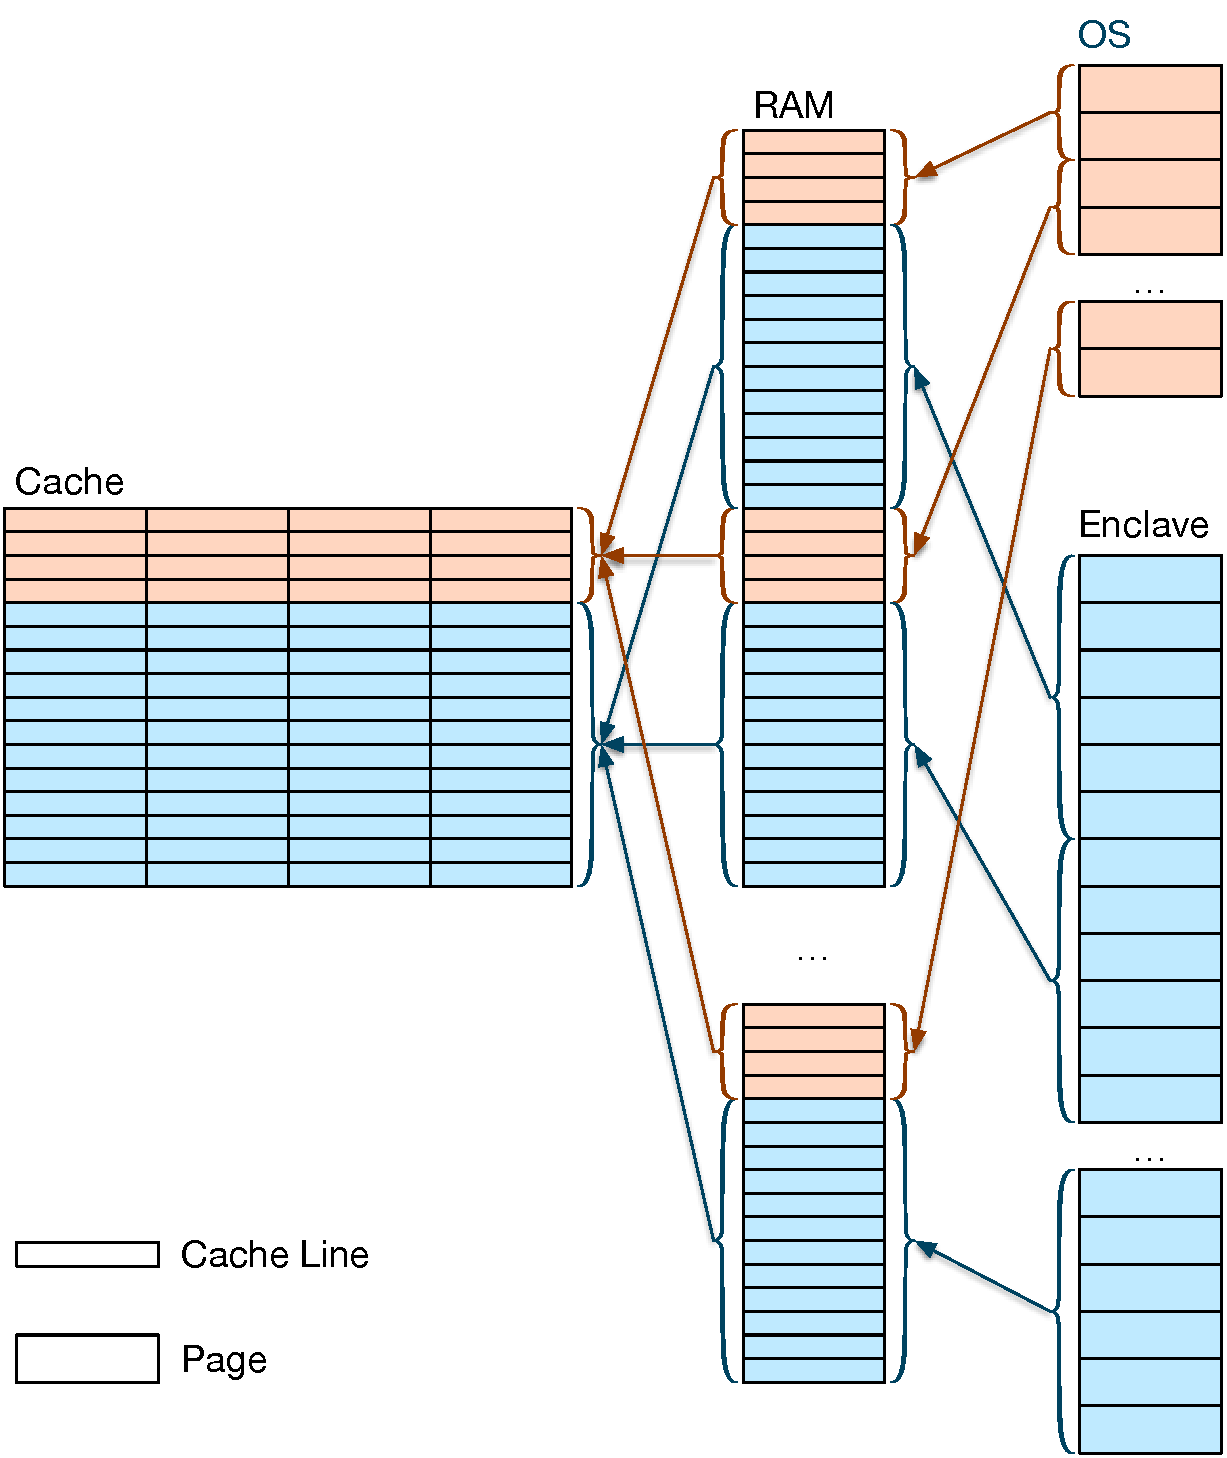
\includegraphics[width=85mm]{figures/cache_partitions.pdf}
  \caption{
    A malicious OS can partition a cache between the software running inside an
    enclave and its own malicious code. Both the OS and the enclave software
    have cache sets dedicated to them. When allocating DRAM to itself and to
    the enclave software, the malicious OS is careful to only use DRAM regions
    that map to the appropriate cache sets. On a system with an Intel CPU, the
    the OS can partition the L2 cache by manipulating the page tables in a way
    that is completely oblivious to the enclave's software.
  }
  \label{fig:cache_partitions}
\end{figure}

The system software stores all the victim enclave's code and data in DRAM
addresses that map to the cache sets in one of the regions, and stores its own
code and data in DRAM addresses that map to the other region's cache sets.  The
snooping thread's code is assumed to be a part of the OS. For example, in a
typical 256~KB (per-core) L2 cache organized as 512 8-way sets of 64-byte
lines, the tracing kernel could allocate lines 0-63 for the enclave's code
page, lines 64-127 for the enclave's data page, and use lines 128-511 for its
own pages.

To the best of our knowledge, there is no minor modification to SGX that would
provably defend against cache timing attacks. However, the SGX design could
take a few steps to increase the cost of cache timing attacks. For example,
SGX's enclave entry implementation could flush the core's private caches, which
would prevent cache timing attacks from targeting them. This measure would
defeat the cache timing attacks described below, and would only be vulnerable
to more sophisticated attacks that target the shared LLC, such as
\cite{yarom2013llctiming, liu2015llctiming}. The description above assumes that
multi-threading has been disabled, for the reasons explained in
\S~\ref{sec:sgx_vs_privileged_sw_attacks}.

Barring the additional protection measures described above, a tracing kernel
can extend the attack described in \S~\ref{sec:sgx_vs_memory_mapping_attacks}
with the steps outlined below to take advantage of cache timing and narrow down the
addresses in an application's memory access trace to cache line granularity.

Right before entering an enclave via \texttt{EENTER} or \texttt{ERESUME}, the
kernel would issue \texttt{CLFLUSH} instructions to flush the enclave's code
page and data page from the cache. The enclave could have accessed a single
code page and a single data page, so flushing the cache should be reasonably
efficient. The tracing kernel then uses 16 bogus pages (8 for the enclave's
code page, and 8 for the enclave's data page) to load all the 8 ways in the 128
cache sets allocated by enclave pages. After an AEX gives control back to the
tracing kernel, it can read the 16 bogus pages, and exploit the time difference
between an L2 cache hit and a miss to see which cache lines were evicted and
replaced by the enclave's memory accesses.

% PRMRR documented in HASP papers and both SGX manuals, completely removed from
% SDM. It still exists in Coreboot. Couldn't find other Skywell code.

% Memory Type Considerations for PRMRR: SGX S 6.11.1, SGX2 S 6.11.1

An extreme approach that can provably defeat cache timing attacks is disabling
caching for the PRM range, which contains the EPC. The SDM is almost completely
silent about the PRM, but the SGX manuals that it is based on state that
the allowable caching behaviors~(\S~\ref{sec:cacheability_config}) for the PRM
range are uncacheable (UC) and write-back (WB). This could become useful if the
SGX implementation would make sure that the PRM's caching behavior cannot be
changed while SGX is enabled, and if the selected behavior would be captured by
the enclave's measurement~(\S~\ref{sec:sgx_measurement}).
